
\documentclass[12pt,a4paper,final]{article}
\usepackage[utf8]{inputenc}
\usepackage[francais]{babel}
\usepackage[T1]{fontenc}
\usepackage{amsmath}
\usepackage{amsfonts}
\usepackage{amsthm}
\usepackage{color}
\usepackage{amssymb}
\usepackage{graphicx}
\usepackage{algorithm}
\usepackage{algorithmic}
\usepackage{fancyhdr}
\usepackage[fs]{umons-coverpage}


%%###### START CHANGE HERE ######
\author{S. Opsommer \& R. Cambier}
\title{Rapport du projet Pac-Man}
\umonsAuthor{\begin{tabular}{lll}
\textsc{Cambier} & Robin & ROBIN.CAMBIERR@student.umons.ac.be\\
\textsc{Opsommer} & Sophie & SOPHIE.OPSOMMER@student.umons.ac.be\\
\end{tabular} }
%% The main title of your thesis
\umonsTitle{Rapport du projet Pac-Man}
%% The sub-title of your thesis
\umonsSubtitle{Projet réalisé dans le cadre \\de la 1ère Master en Sciences Informatiques \\pour le cours de \og Software Evolution \fg}
%% Your supervisor(s)
\umonsSupervisor{\begin{tabular}{ll}
\textit{Titulaire} : & T. \textsc{Mens} \\
\textit{Assistant} : & M. \textsc{Claes} \\
\end{tabular}}
%% The date (or academic year)
\umonsDate {\hfill Ann\'ee Acad\'emique 2014-2015}
%%###### END CHANGEMENT ######

\newcommand{\smalltitle}[1]{\bigskip\large\textbf{#1}\par\normalsize\medskip}
\newcommand{\partitle}[1]{\bigskip\textit{\underline{#1}}\par\medskip}
\newcommand{\annexe}[1]{annexe~\ref{#1} (page~\pageref{#1})}
\newcommand{\labelfigure}[1]{figure~\ref{#1} (page~\pageref{#1})}

\graphicspath{{images/}}

\newtheorem{defi}{Définition}
\newtheorem{note}{Note}
\newtheorem{prop}{Propriété}
\newtheorem{exemple}{Exemple}
\newtheorem{corollaire}{Corollaire}
\newtheorem{lemme}{Lemme}
\newtheorem{rem}{Remarque}
\newtheorem{thm}{Théorème}

\fancyhf{}
\chead{\leftmark}
\rfoot{\thepage}

\begin{document}

\umonsCoverPage
\pagebreak

\pagestyle{fancy}

\thispagestyle{empty}
\newpage
\tableofcontents
\newpage

%%###### LE RAPPORT COMMENCE ICI ######
\thispagestyle{empty}
%\smalltitle{......}
\vspace*{\stretch{1}}
\begin{abstract}
\addcontentsline{toc}{section}{Résumé}
Ce \emph{rapport} est rendu dans le cadre du cursus de première année de \og Master en Sciences Informatiques\fg  pour le cours de \emph{Software Evolution} (dont le titulaire est Mr. \emph{T. Mens} et l'assistant est Mr. \emph{M. Claes} en année académique 2014-2015) . Le but de ce rapport est de présenter les résultats de la réalisation du projet Pac-Man.
\end{abstract}
\vspace*{\stretch{1}}

\newpage
\section{Introduction}\label{sec:intro}
\subsection{Problème posé}
A partir d'un code existant, ce projet consiste à : 
\begin{itemize}
\item analyser la qualité du logiciel, en utilisant des techniques d'analyse statique du code (par exemple, la détection du code dupliqué et des bad smells, les diverses métriques de qualité) et les outils d'analyse dynamique du code (par exemple, le profilage, la couverture du code et des tests);
\item améliorer la qualité et la structure du code (en utilisant des refactorings, en introduisant des design patterns, et en modularisant le code) ;
\item étendre le logiciel avec de nouvelles fonctionnalités (évolution), et étudier l'effet de cela sur la qualité du code;
\item tester le logiciel avant et après chaque modification. Ceci implique que vous devez ajouter des tests unitaires (unit tests) pour au moins les fragments du code modifiés ou ajoutés, et d'appliquer des tests de régression à chaque modification.
\end{itemize}

\subsection{Etapes clés}
Les étapes clés du projet sont les suivantes : (chronologiquement)
\begin{enumerate}
\item Analyse de la qualité de la premiére version du code (section \ref{etape1})
\item Ajout de tests unitaires à la première version du code (section ...), et vérification de la couverture des tests
\item Refactoring du code pour en améliorer la qualité et la structure (section ...)
\item Analyse des améliorations de qualité et tests de régression (section ...)
\item Extension du logiciel et ajout des tests unitaires pour cette extension (section ...)
\item Analyse de la qualité de cette extension et tests de régression (section ...)
\item Etude de l'historique de la qualité logicielle entre toutes les versions du code (section ...)
\end{enumerate}
%%%%%%%%%%%%%%%%%%%%%%%%%%%%%%%%%%%%%%%%%%%%%%%%%%%%%%%%%%%%%%%%%%%%%%%%%%%%%%%%%%
\section{Etape 1 : Première analyse de la qualité du logiciel }\label{sec:etape1}
\subsection{Enoncé}
Le but de la première étape clé est d'analyser la qualité du logiciel pour avoir une première idée de ce qu'il faudra corriger si l'on désire améliorer la qualité. Cette première analyse est également l'occasion de comprendre l'architecture et la dynamique du système.
Pour cette étape clé il est demandons de :
\begin{enumerate}
\item Calculer la valeur de plusieurs métriques logicielles permettant d'estimer la qualité du logiciel, d'interpréter les résultats des métriques, et de mettre en évidence les modules (packages, classes ou méthodes) qui devraient être traités prioritairement afin d'améliorer leur qualité ainsi que la raison pour laquelle ils sont prioritaires.
\item Déterminer les classes et les méthodes qui sont couvertes par des tests unitaires, et mettre en évidence les méthodes pour lesquelles de nouveaux tests unitaires devraient être créés prioritairement.
\item Répertorier les portions de code qui ne sont pas utilisées et qui pourraient donc être supprimées sans altérer le comportement du système.
\item Répertorier les portions de code qui sont redondantes (code dupliqué) et qui pourraient donc être éliminées par une restructuration du système sans altérer son comportement.
\item Détecter la présence de bad smells. En trouvez-vous une plus forte concentration dans certains modules ?
\item Analyser les performances du système en terme d'utilisation CPU et de consommation de mémoire. Repérez les parties du code créant un goulot d'étranglement et précisez les modules qui devraient être retravaillés afin de procéder à un déoulottage du système.
\end{enumerate}
Décrivez la qualité globale du système. Quel serait, selon vous, le coût nécessaire à sa maintenance et à son évolution ?
%%%%%%%%%%%%%%%%%%%%%%%%%%%%%%%%%%%%%%%%%%%%%%%%%%%%%
\subsection{Résultat}

\subsubsection{Code dupliqué}\label{codeduplique}
Du code dupliqué consiste à trouver au sein d'un projet des blocs de lignes de code identique en plusieurs exemplaires.
C'est un facteur de mauvaise qualité parce que ça rend le code plus difficile à changer, à maintenir, à comprendre,...
Les solutiuons qui sont offertent par les languages de programmation sont les méthodes, les fonctions, les librairies, l'encapsulation des objets.
Eviter de dupliquer du code permet d'avoir un programme plus cohésif.

\begin{figure}[!h]
	\centering
	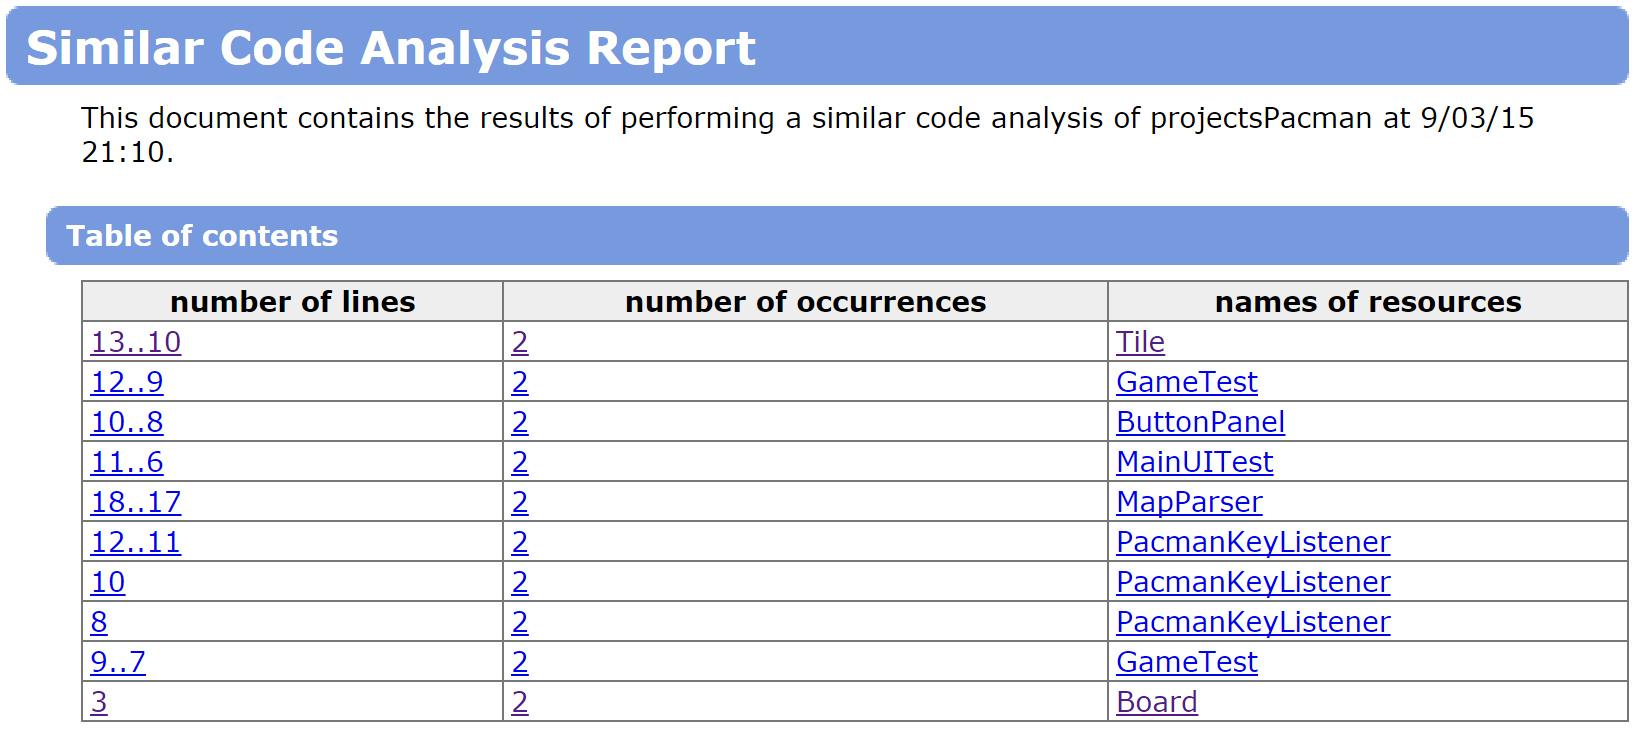
\includegraphics[width=\textwidth]{SimilarCode_00.png}
	\caption{\label{SimilarCode0}Résultat de l'analyse de "code dupliqué" par CodePro}
\end{figure}

Pour analyser cette métrique, nous avons utiliser le programme CodePro à partir de l'interface d'Eclipse ( Eclipse -> CodePro Tools -> Find Similar Code).
Nous pouvons observer sur la \labelfigure{SimilarCode0} que cet outils a détécté 10 blocs de code. Les figures de l'\annexe{SimilarCode} permettent de visualiser les différents blocs de code.
Les classes concernées sont : Tile.java, GameTest.java, ButtonPanel.java, MainUITest.java, MapParser.java, PacmanKeyListener.java, PacmanKeyListener.java, PacmanKeyListener.java,  GameTest.java, Board.java.

Ce résultat n'est pas bon, mais on peut observer que les blocs se trouve chaque fois dans une même classe. Il sera donc probablement possible de créer des fonction pour chacun de ses cas.



\subsubsection{Dépendences cycliques}\label{dépendances}
Une dépendance cyclique peut-être appelée dépendance cyclique directe ou indirecte et elle a la même difinition qu'il s'agisse de dépendances entre des projets, entre des packages ou entre des classes. Quand on a une dépendance directe, on a un élément X qui dépend d’un élément Y qui dépend lui-même de X. Contrairement à la dépendance cyclique indirecte où la situation dans laquelle on se trouve est tel que X dépend de Y, Y dépend de Z et Z dépend de X.
Du point de vue de la compilation, plus une dépendance est haut niveau, plus elle est à traiter en priorité. En effet entre deux classes, ce n'est pas très grave et ça ne pose généralement pas de problème. Entre deux package c'est fortement déconseillé même s'il est généralement possible de compiler le projet. Par contre entre deux projets, l'issue est fatale puisque chaque projet doit-être compilé avant de pouvoir compiler l'autre.
Du point de vue de la maintenance, une dépendance d'un élément A à un élément B et vice-versa impose que pour pouvoir modifier A, il faut commencer par modifier B et pour pouvoir modifier B, il faut commencer par retravailler B. L'évolution de ses éléments est donc compliquée.

Pour pallier à ce genre de problème, plusieurs pistes sont possible : déplacer les éléments (les classes si le problème concerne deux packages ou la(les) méthodes si le soucis se situe entre deux classes), redécouper certaines éléments (pour mieux associer les blocs de code aux éléments qui en ont besoin), regrouper les éléments (pour n'en former plus qu'un seul),... %pistede solution à l'adresse  :http://blog.developpez.com/wichtounet/p8723/jtheque/osgi_et_dependances_cycliques

\begin{figure}[!h]
	\centering
	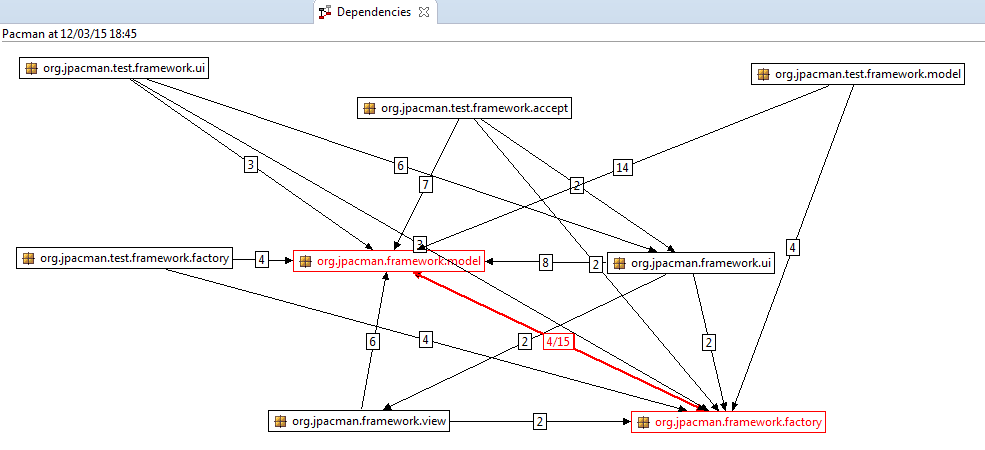
\includegraphics[width=\textwidth]{DependenciesPackages.png}
	\caption{\label{dependenciesPackage}Détail de l'analyse des dépendences cycliques des packages du projet.}
\end{figure}
\begin{figure}[!h]
	\centering
	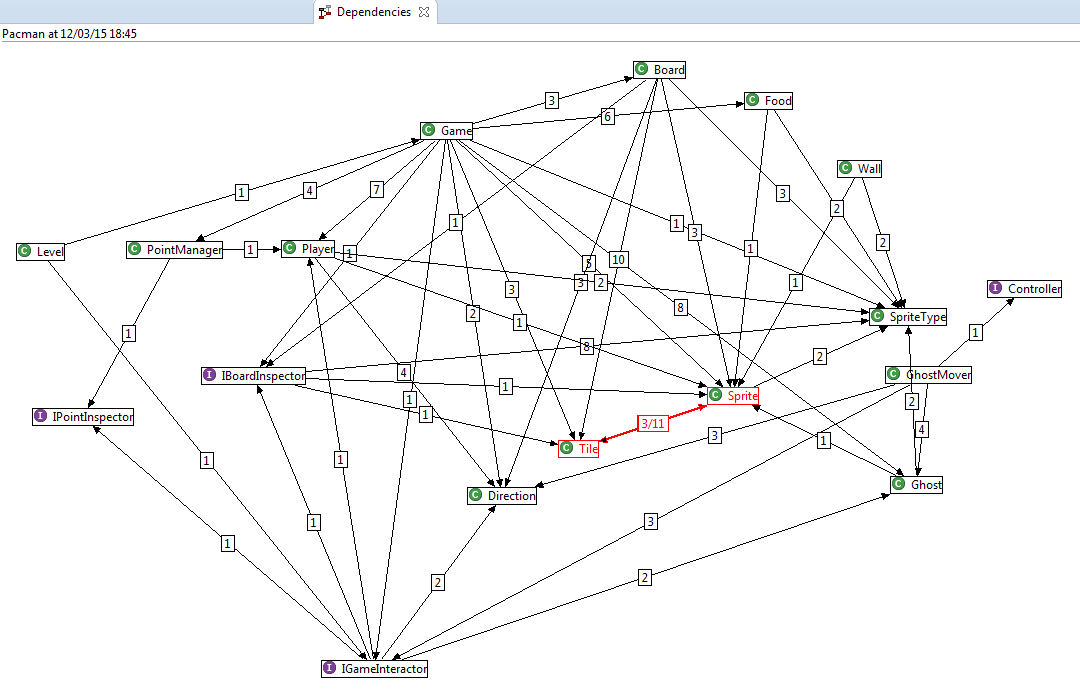
\includegraphics[width=\textwidth]{DependenciesModel.png}
	\caption{\label{dependenciesModel}Détail de l'analyse des dépendences cycliques du package Model.}
\end{figure}

Cet métrique a aussi été visualisée à partir de l'outil CodePro depuis Eclipse (Eclipse -> CodePro Tools -> Analyse Dependencies).
On peut observer sur la \labelfigure{dependenciesPackage} et la \labelfigure{dependenciesModel} qu'il existe des dépendences cycliques au sein du package Model (entre les classes Sprite et Tile) et entre le package Model et le package Factory.
L'\annexe{Dependencies} contient toutes les autres visualisations qui n'ont pass révélé de problème de dépendances.


\subsubsection{Code inutile}
Du code inutile, aussi appelé "Dead Code", correspond à des lignes de code qui sont compilée mais qui ne sont jamais utilisée. 
C'est fréquement du code qui a été utile à une fonctionnalité et lorsque cette fonctionnalité à été supprimée/ réécrite, déplacée,... ce code est resté.
Le problème dans ce cas est que ça ralentit la compréhension du développeur lors de la lecture, ça gaspille des ressources au compilateur et lors de l'éxécution.
La solution est généralement de supprimer ses lignes de code.

\begin{figure}[!h]
	\centering
	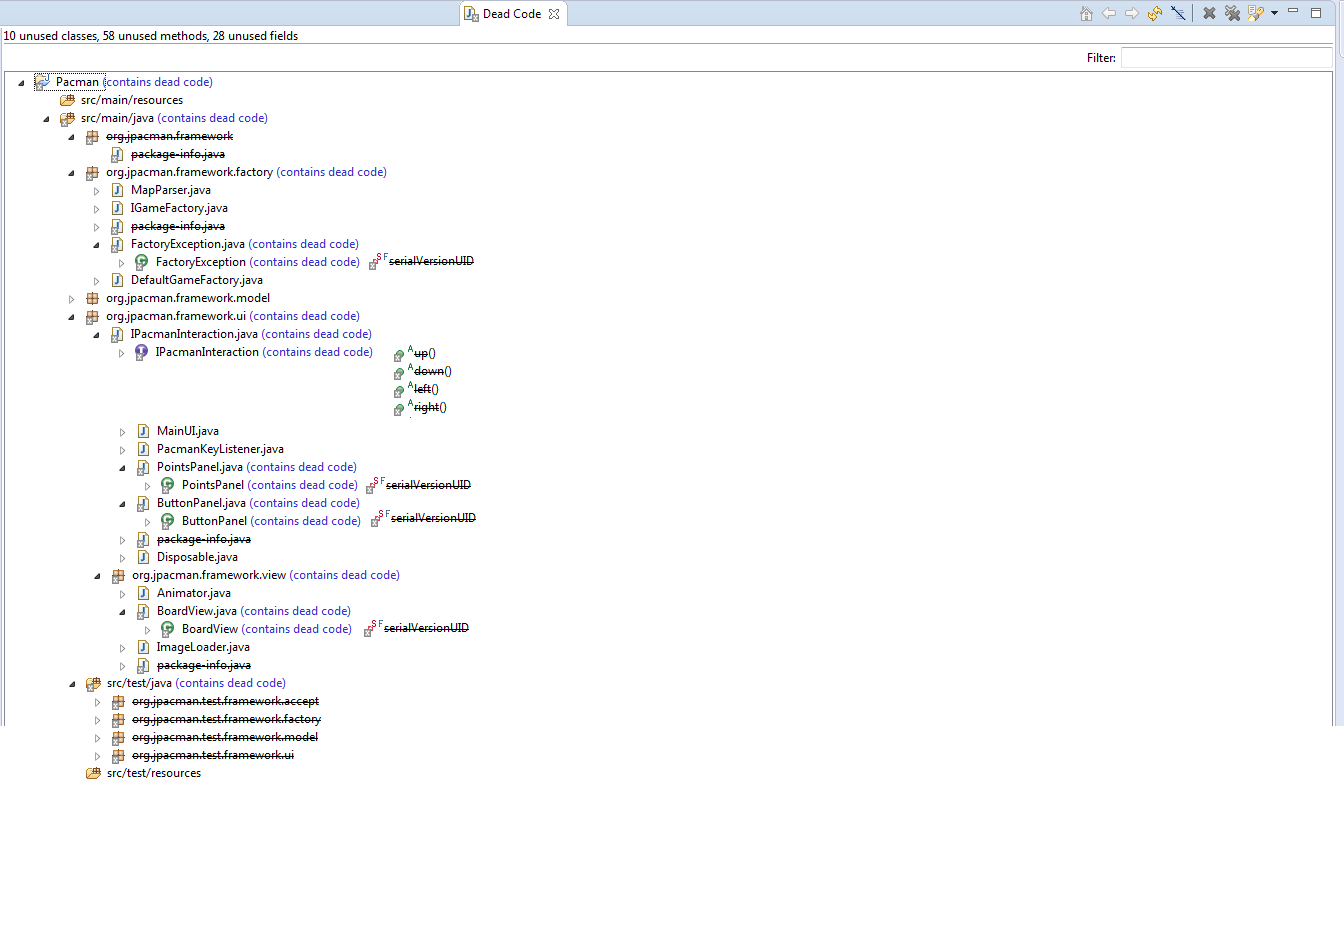
\includegraphics[width=\textwidth]{DeadCode.png}
	\caption{\label{deadcode}Détail de l'analyse des parties de code non utilisé lors de l'éxécution du programme.}
\end{figure}

L'outil utilisé reste CodePro depuis Eclipse (Eclipse -> CodePro Tools -> Find dead code).
Attention tout de même à ne pas tout supprimer sans réfléchir, en effet, on observer sur la \labelfigure{deadcode} que les packages contenant les test sont considéré comme inutile. Ils le sont en effet lors de l'éxécution du programme, mais ne le sont pas au bon développement du programme.
Il en va de même pour les variables "`serialVersionUID"'. Ces variables, bien que inutile lors de l'exécution, doivent-être présente dans les classes qui étendent (directement ou indirectement) la classe "`Sérializable"'. Leur valeur est indispensable pour des applications qui transittent par le réseau mais leur existence ne peut causer aucun tort.
Pour ce qui est des fichiers "`package-info.java"', il sont a nouveau inutule lors de l'exécution du code, mais permettent de contenir les commentaires contenant l'information relative au package en vue de la création de la javadoc. Ces fichiers sont donc à conservr (et à complêter dans certains cas).
Les modifications à éffectuées ici sont donc mineures.


\subsubsection{Javadoc}
La javadoc est une documentation standard au format HTML pour les programmes developpé en JAVA. Elle est créée de façon automatique par la plupart des outils de développement en se basant sur les tags placés dans le code au dessus de la déclaration de chaque classe et de chaque méthode (pour la documentation des packages, elle se trouve dans les fichiers "`paquage-info.java"').
L'utiliser est un plus mais ne consiste en rien en une obligation (mais alors il sera tout de même fortement conseillé d'utiliser les commentaires classique pour constituer un code suffisemment documenter à la compréhension).

Grace à l'outil CodePro d'Eclipse, il a été observé (non illustré parce que toutes les classes sont a revoir) que en règle générale, les classes sont documentée. L'outil détecte bien quelques manquement, mais ce sont généralement l'un ou l'autre tag qu'il détecte manquant mais qui ne perturbe pas la compréhension ainsi que les classes DefaultGameFactory, Game, IBoardInspector, IPointInspector, Player et PointManager dont les méthodes ne sont pas commentée et les méthodes issues d'une interface (sous l'annotation "`@Overhide"').

\subsubsection{}


\subsubsection{Test unitaire}
Cet analyse sera détaillée dans la section suivante \ref{etape2}.


%Respect des conventions de codage
%Performances
%Structure du code
%Style du code
%Design flaws
%Antipattern
%Test
%Dataflow 
%Documentation
%Profilage

\subsubsection{Outils généraux}
Il est important de signaler aussi, que l'outil Eclipse soulève certaines attention à l'aide de "`warnings"',  

Les types d'erreurs : 
\begin{itemize}
\item Empty block should be documented x2
\item Javadoc: Missing comment for public declaration x 51
\item Redundant specification of type arguments <...> x6
\item The import ... is never used x4
\item The method ... of type ... should be tagged with @Override since it actually overrides a superinterface method x13
\item The parameter ... is hiding a field from type ... x 7
\end {itemize}

Leurs emplacements : \\
\begin{tabular}{|l|l|l|l|}
\hline
Package & \# warning & Classe & \# warnings \\
\hline
/main/java/.../model & 60 & Game.java & 15 \\
&& IBoardInspector.java & 13 \\
&& Direction.java & 8 \\
&& Player.java & 7 \\
&& Board.java & 4 \\
&& IPointInspector.java & 3 \\
&& PointManager.java & 3 \\
&& Tile.java & 3 \\
&& GhostMover.java & 2 \\
&& Sprite.java & 1 \\
&& Food.java & 1 \\
\hline
/main/java/.../ui & 15 & ButtonPanel.java & 8 \\
&& PacmanKeyListener.java & 5 \\
&& MainUI.java & 2 \\
\hline
/test/java/.../model & 5 & SpriteTest.java & 5 \\
\hline
main/java/.../factory & 2 & MapParser.java & 2 \\
\hline
/test/java/.../ui & 1 & MainUIFocusTest.java & 1 \\
\hline
\end{tabular}

Et grace à l'outil de calcul des métrique, on peut observer : 
%%%%%%%%%%%%%%%%%%%%%%%%%%%%%%%% Pq elles s''affichent pas ??????????  !!!!!!!!!!!!!!!!!!!!!!!!!!!!!!!!!!!!!!!!!!!!!!!!
\begin{figure}[!h]
	\centering
	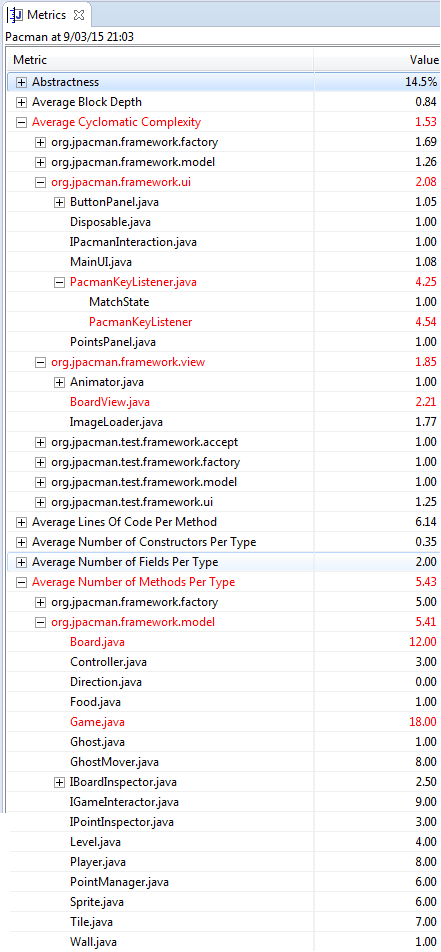
\includegraphics[width=\textwidth]{Metrique.png}
	\caption{\label{métrique0}Suite des détails de l'analyse des métriques du projet.}
\end{figure}

\begin{figure}[!h]
	\centering
	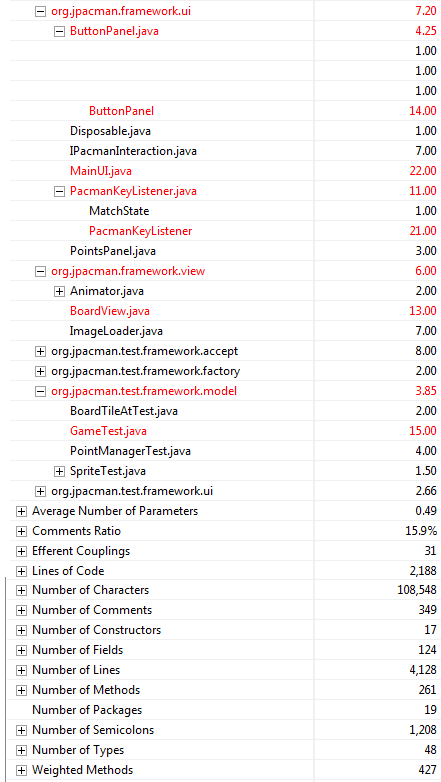
\includegraphics[height=\textheight]{Metrique_.png}
	\caption{\label{métrique0}Suite des détails de l'analyse des métriques du projet.}
\end{figure}

%%%%%%%%%%%%%%%%%%%%%%%%%%%%%%%%%%%%%%%%%%%%%%%%%%%%%%%%%%%%%%%%%%%%%%%%%%%%%%%%%%
\newpage
\section{Etape 2 : Ajout de tests unitaires}\label{sec:etape2}
\subsection{Enoncé}
Votre première analyse a révélé la présence de certains problèmes de qualité du code de l'application.
Avant d'envisager la correction de ces problèmes, il faut s'assurer que les modifications que vous apporterez au code source ne modifieront pas le comportement du logiciel.
Etendez et complétez le jeu de tests unitaires fourni avec le code source afin de vous prémunir d'une telle modification. Effectuez également une analyse de couverture de tests.
Quelle garantie avez-vous que vos futures modifications ne pourront pas casser le système ?

\subsection{Résultat}

Tests  Eclipse -> Coverage As -> JUnit Test : La figure \annexe{coverage} montre que le projet est couvert à $68.3 \%$ avec en particulier, $63.5\%$ pour la package \emph{main} et $83.7\%$ pour le package \emph{test}.
 Il est donc important d'ajouter des tests sur les classes : FactoryException, Board, Sprite et PacmanKeyListener qui sont sous le seuil des $50 \%$ de couverture.

%%%%%%%%%%%%%%%%%%%%%%%%%%%%%%%%%%%%%%%%%%%%%%%%%%%%%%%%%%%%%%%%%%%%%%%%%%%%%%%%%%
\newpage
\section{Etape 3 : Refactoring en vue d'améliorer la qualité}\label{sec:etape3}
\subsection{Enoncé}
Avec les tests unitaires ajoutés dans l'étape précédente, vous pouvez vérifier automatiquement (jusqu'à un certain point) la préservation du comportement du logiciel. Réalisez les modifications nécessaires à l'amélioration de la qualité et la structure du logiciel. 
Vos ressources et votre temps étant limités, commencez par établir les modifications devant être réalisées en priorité. Sur base de quels critères réalisez-vous cette priorisation ?
Refactorisez progressivement votre code, en vous assurant systématiquement que tous les tests déjà présents s'exécutent avec succès. Souvenez-vous que vos modifications doivent améliorer la qualité du code, et non étendre ou modifier le comportement du logiciel.

\subsection{Résultat}



%%%%%%%%%%%%%%%%%%%%%%%%%%%%%%%%%%%%%%%%%%%%%%%%%%%%%%%%%%%%%%%%%%%%%%%%%%%%%%%%%%
\newpage
\section{Etape 4 : Analyse de la qualité du logiciel}\label{sec:etape4}
\subsection{Enoncé}
Réalisez une étude similaire à celle décrite en Section ... La qualité du logiciel s'est-elle améliorée ? Les problèmes les plus critiques ont-ils été résolus ? Au vu de cette seconde analyse, quels sont les points qui devraient à présent être améliorés ?
\subsection{Résultat}



%%%%%%%%%%%%%%%%%%%%%%%%%%%%%%%%%%%%%%%%%%%%%%%%%%%%%%%%%%%%%%%%%%%%%%%%%%%%%%%%%%
\newpage
\section{Etape 5 : Extensions}\label{sec:etape5}
\subsection{Enoncé} 
Il vous est demandé d'étendre le logiciel afin d'y ajouter certaines fonctionnalités ou d'en améliorer la qualité. Chaque équipe doit réaliser au moins deux extensions diférentes, décrites dans la section ... .
Utilisez un processus de développement dirigé par les tests (test-driven development) : lors du développement des extensions, ajoutez de nouveaux tests unitaires pour tester le comportement prévu de l'extension. Effectuez également des tests de régression avec les tests unitaires déjà présents, afin de vous assurer que le comportement initial n'a pas été modifié.
\subsection{Résultat}



%%%%%%%%%%%%%%%%%%%%%%%%%%%%%%%%%%%%%%%%%%%%%%%%%%%%%%%%%%%%%%%%%%%%%%%%%%%%%%%%%%
\newpage
\section{Etape 6 : Analyse de la qualité du logiciel}\label{sec:etape6}
\subsection{Enoncé} 
Pour chaque extension ajoutée, réalisez une analyse de qualité similaire à celle décrite en Section ... Au vu de cette analyse, quels sont les points qui devraient à présent être améliorés ?
\subsection{Résultat}



%%%%%%%%%%%%%%%%%%%%%%%%%%%%%%%%%%%%%%%%%%%%%%%%%%%%%%%%%%%%%%%%%%%%%%%%%%%%%%%%%%
\newpage
\section{Etape 7 : Analyse de l'évolution de la qualité logicielle}\label{sec:etape7}
\subsection{Enoncé} 
Analysez l'évolution de la qualité du logiciel entre les diférentes versions, en utilisant les résultats d'analyse de qualité des sections ..., ... et ... . Montrez cette évolution graphiquement et interprètez-la.
\subsection{Résultat}







%%%%%%%%%%%%%%%%%%%%%%%%%%%%%%%%%%%%%%%%%%%%%%%%%%%%%%%%%%%%%%%%%%%%%%%%%%%%%%%%%%
Quelque exemple d'utilisation. \textit{"Un peu d'italique"} \textbf{Du Gras}. Pour séparer deux paragraphe il suffit de mettre deux enter (une ligne blanche en gros)

Et voila un nouveau paragraphe :)\\
On peut egalement simplement revenir en arriere comme ca \\

Une petite liste a puce ? numéroté?

\begin{itemize}
\item $V$ est un ensemble fini de noeuds
\item $E$ est un ensemble d'arcs reliant deux noeuds
\end{itemize}

\begin{enumerate}
\item Remplacer la valeur de la racine par celle du dernier noeud, celui qui sera le plus à droite de la dernière ligne (le "1" dans l'exemple de la figure~\ref{heapExample}(a)).
\item Supprimer ce dernier noeud
\item Faire redescendre tant que nécessaire la nouvelle racine.
\end{enumerate}
Une image ? Avec une reference dans un texte ? no probleme :p

Un graphe orienté est défini par un couple: $G=(V,E)$.
La figure~\ref{graphExample} illustre un graphe.

La complexité c'est pas un simple O(lg n) mais $\mathcal{O}(\log_2 n)$.\\

\smalltitle{un petit titre qui n'apparait pas dans la table des matiere}
blablabla

\partitle{encore un plus petit titre}
blablabla

Un algorithme ? ouille ouille ouille :p mais on si habitue. Le caption sera le titre visible et le label sera ce que tu devra utiliser pour le referencer comme ca Alogo~\ref{extractMin}

%\begin{algorithm}[H]
%\caption{extractMin($A$)}\label{extractMin}
%\begin{algorithmic}[1]
%\STATE $min\gets A[1]$
%\STATE $A[1]\gets A[A.heapsize]$
%\STATE $A.heapsize\gets A.heapsize - 1$
%\STATE heapify($A, 1$)
%\end{algorithmic}
%\end{algorithm}

%\begin{algorithm}[H]
%\caption{heapify($A,i$)}\label{heapify}
%\begin{algorithmic}[1]
%\STATE $l\gets $left($i$)
%\STATE $r\gets $right($i$)
%\IF{$l \leq A.heapsize$ \AND $A[l] < A[i]$ }
%\STATE $smallest\gets l$
%\ELSE
%\STATE $smallest\gets i$
%\ENDIF
%\IF{$r <leq A.heapsize$ \AND $A[r] < A[smallest]$}
%\STATE $smallest\gets r$
%\ENDIF
%\IF{$i \neq smallest$}
%\STATE switch($A[i], A[smallest]$)
%\STATE heapify($A, smallest$)
%\ENDIF
%\end{algorithmic}
%\end{algorithm}

%\begin{algorithm}[H]
%\caption{decreaseKey($A,i,key$)}\label{heapify}
%\begin{algorithmic}[1]
%\IF{$key > A[i]$}
%\STATE \textbf{error} "la nouvelle clé doit être inférieur à la valeur actuel"
%\ENDIF
%\STATE $A[i]\gets key$
%\WHILE{$i>1$ \AND $A[$parent($i$)$] > A[i]$}
%\STATE switch($A[i],A[$parent($i$)$]$)
%\STATE $i\gets $parent($i$)
%\ENDWHILE
%\end{algorithmic}
%\end{algorithm}

Des theorme, lemme, propriete ? sa marche aussi :). De nouveaux tu peux reference le label :) Lemme~\ref{upper-bound_prop}

\begin{lemme}[Propriété de borne supérieur]\label{upper-bound_prop}
Nous avons à tout moment $v.d \geq \delta(s,v) \forall v \in V$, et une fois que $v.d$ atteins $\delta(s,v)$ il ne changera plus.
\end{lemme}

\begin{corollaire}[Propriété d'absence de chemin]\label{no_path_prop}
Si il n'existe pas de chemin allant de $s$ à $v$ alors nous avons à tout moment $v.d = \delta(s,v) = \infty$.
\end{corollaire}

\begin{prop}[Propriété de convergence]\label{convergence_prop}
Si $s \leadsto u \rightarrow v$ est un plus court chemin dans $G$ pour $u, v \in V$ donné et si $u.d = \delta(s,u)$ avant que l'arc ($u,v$) ne soit relaxé alors $v.d = \delta(s,v)$ après la relaxation.
\end{prop}

\begin{thm}[Thm de convergence]\label{convergence_thm}
Si $s \leadsto u \rightarrow v$ est un plus court chemin dans $G$ pour $u, v \in V$ donné et si $u.d = \delta(s,u)$ avant que l'arc ($u,v$) ne soit relaxé alors $v.d = \delta(s,v)$ après la relaxation.
\end{thm}

des symbole grec, mathematique $\delta(a), \sigma(a), \neq, \leq, \geq, ...$\\
Ca doit etre entre dollard. Pareil pour toutes les variables, formule, ...\\
on n'ecrit pas l'index i mais l'index $i$





\clearpage
\newpage
\section{Annexes} \label{sec:annexe}
\appendix %permet de changer la numérotation en lettre
\section{Annexe : Code Dupliqué}\label{SimilarCode}
Dans cette section se trouve les différentes annexes qui permettent d'identifier les blocs de dode dupliqués détecté par CodePro. Les images illustres les blocs de code. La dernière image illustres les 6 derniers blocs de code et est issue du rapport généré par CodePro (parce que Eclipse les masque).
N.B. : La figure repprennant tous les blocs identifié se trouve à la sous-section \ref{codeduplique}

\begin{figure}[ht]
	\centering
	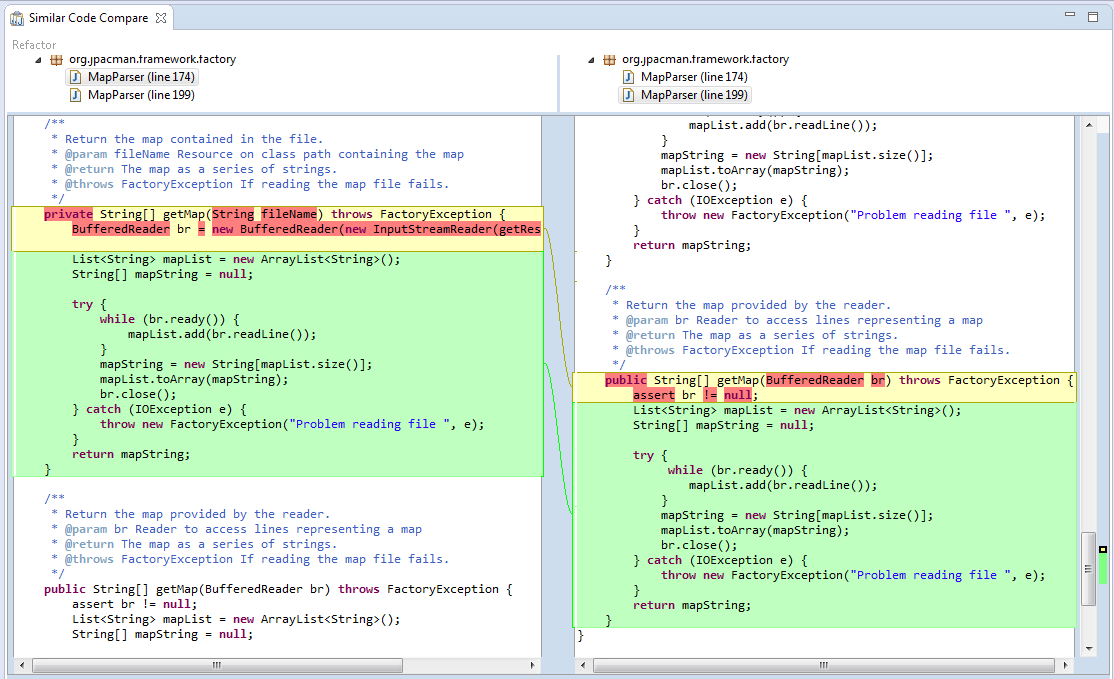
\includegraphics[width=\textwidth]{images/SimilarCode_1.png}
	\caption{\label{SimilarCode1}Détail de l'analyse de code redondant par CodePro}
\end{figure}

\begin{figure}[ht]
	\centering
	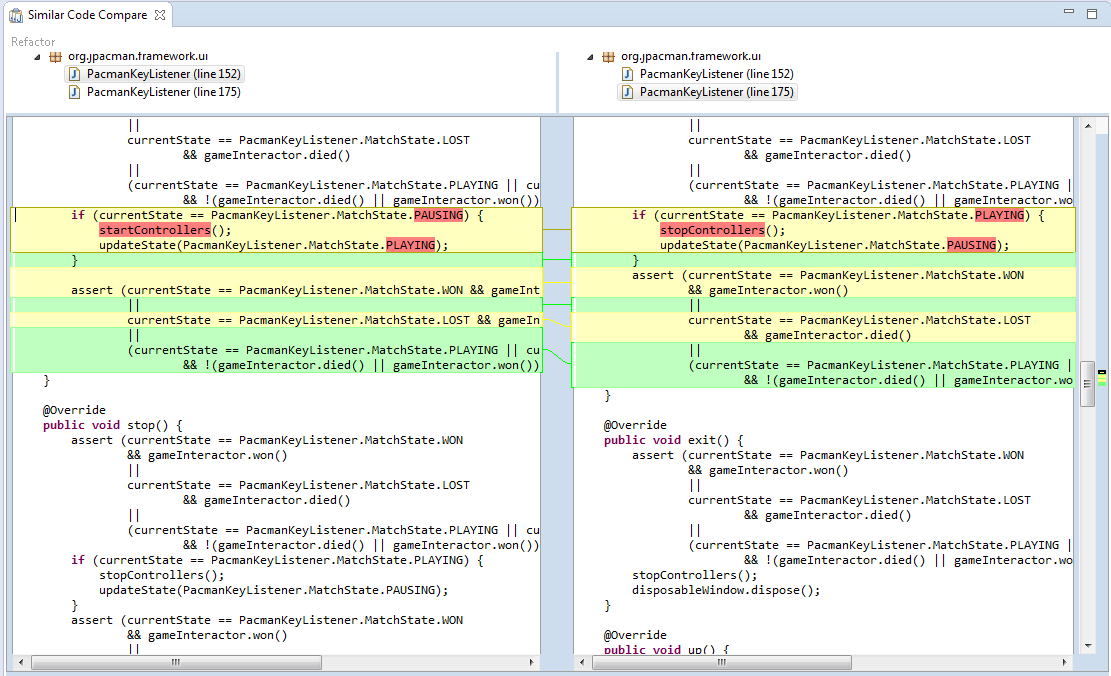
\includegraphics[width=\textwidth]{images/SimilarCode_2.png}
	\caption{\label{SimilarCode2}Détail de l'analyse de code redondant par CodePro}
\end{figure}

\begin{figure}[ht]
	\centering
	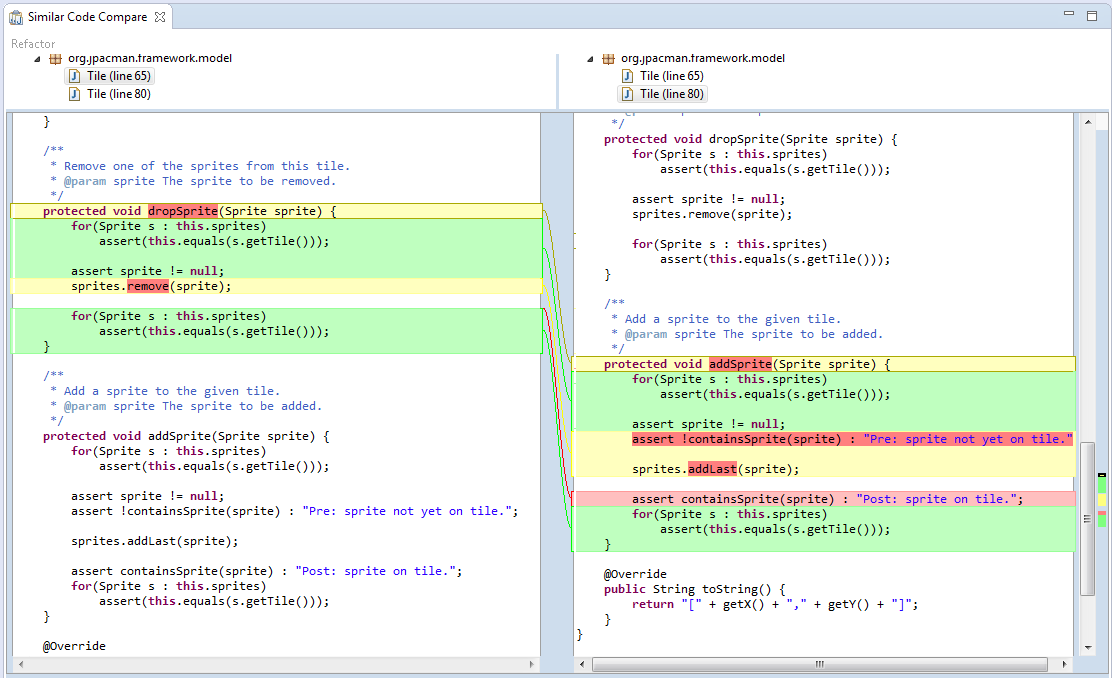
\includegraphics[width=\textwidth]{images/SimilarCode_3.png}
	\caption{\label{SimilarCode3}Détail de l'analyse de code redondant par CodePro}
\end{figure}

\begin{figure}[ht]
	\centering
	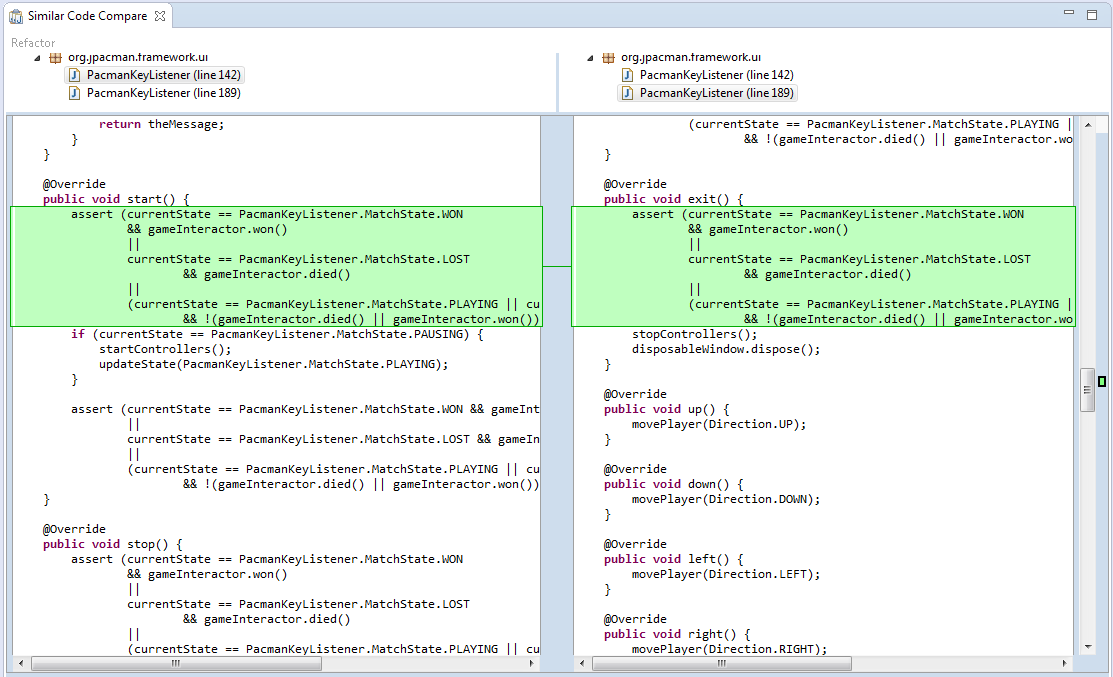
\includegraphics[width=\textwidth]{images/SimilarCode_4.png}
	\caption{\label{SimilarCode4}Détail de l'analyse de code redondant par CodePro}
\end{figure}

\begin{figure}[ht]
	\centering
	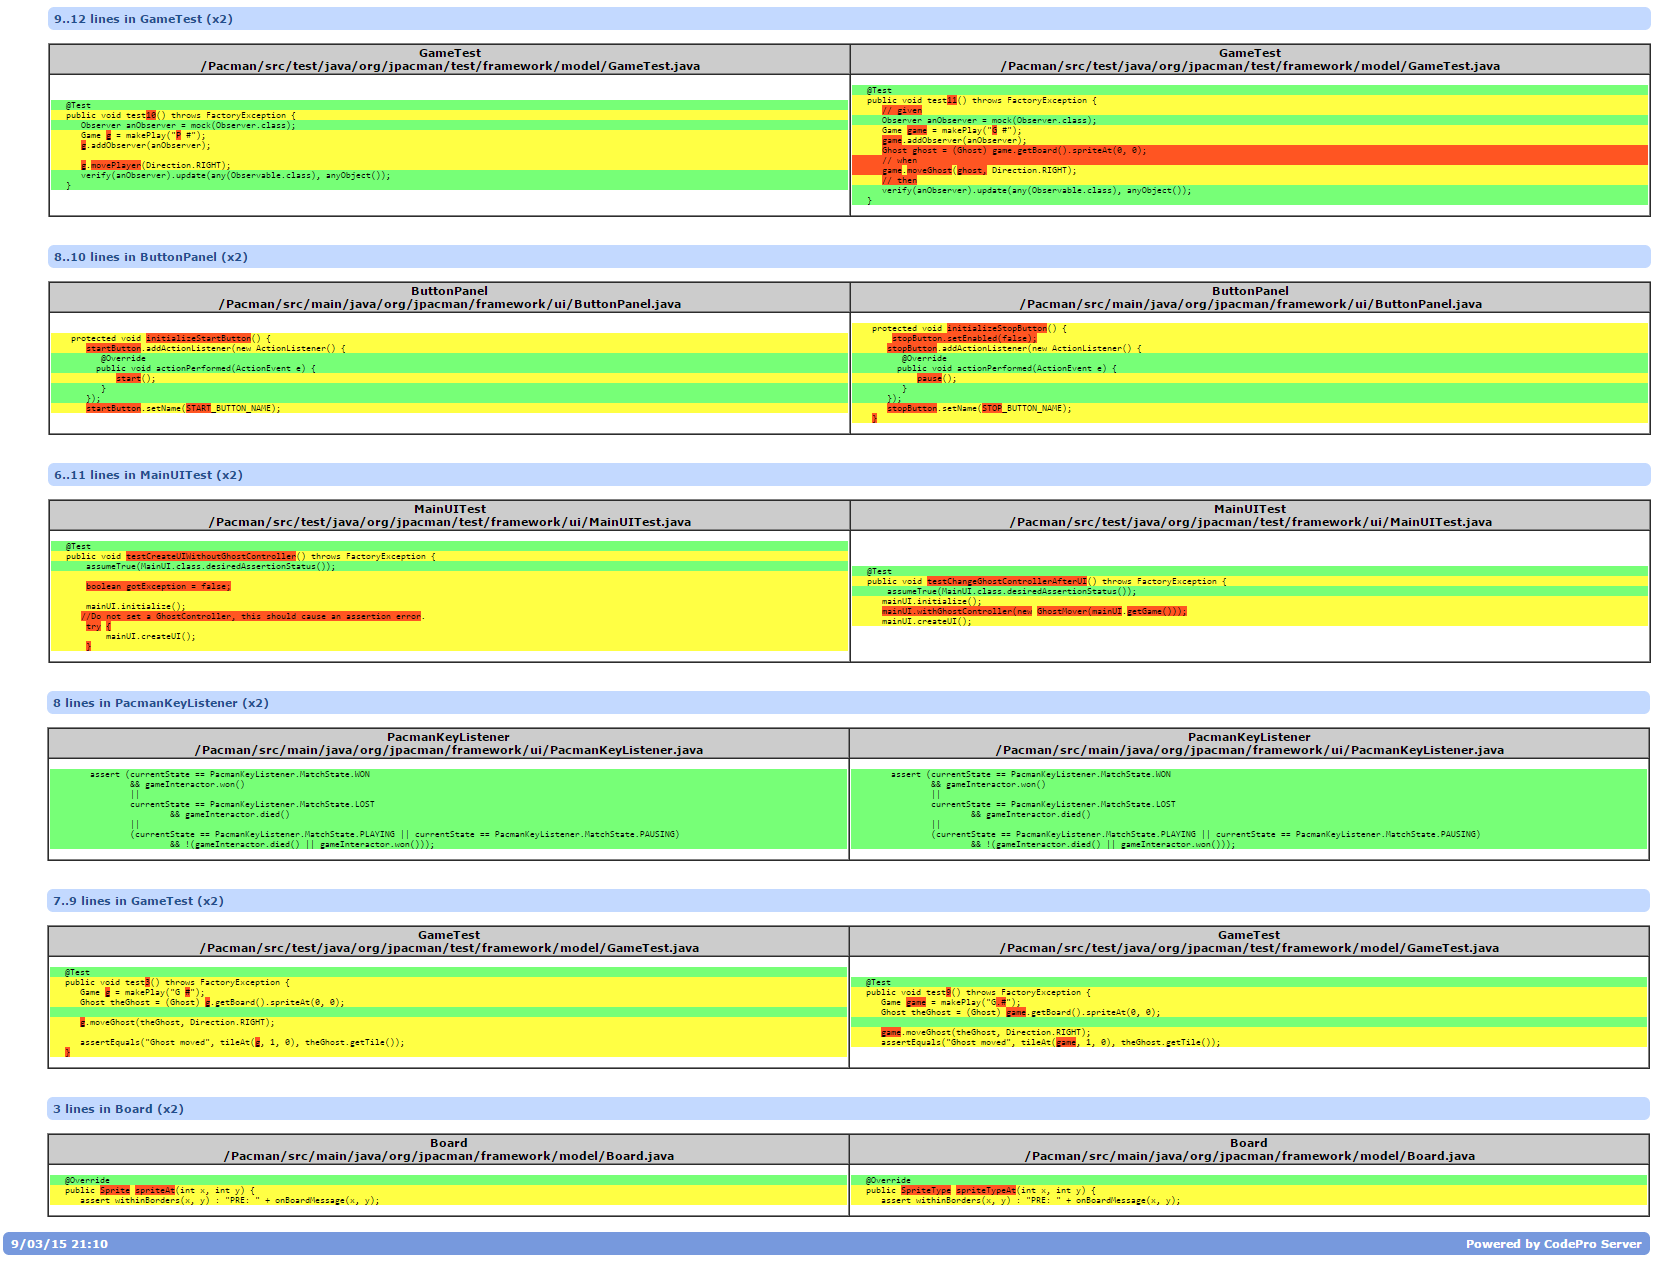
\includegraphics[width=\textwidth]{images/SimilarCode_5.png}
	\caption{\label{SimilarCode5}Détail de l'analyse de code redondant par CodePro (élément dont la visualisation n'est pas possible dans Eclipse)}
\end{figure}

\clearpage
\newpage
\section{Annexe : Dépendances}\label{Dependencies}
Ces figures permettent de visualiser les dépendances entre les différents éléments du projet.
N.B. : Les figures des dépendances entre les packages et des dépendances au sein du package Model se trouve  à la sous-section \ref{dépendances}.

\begin{figure}[ht]
	\centering
	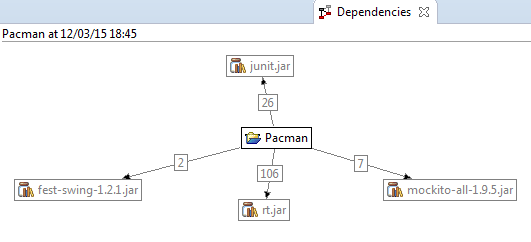
\includegraphics[width=\textwidth]{images/DependenciesProject.png}
	\caption{\label{dependenciesP}Détail de l'analyse des dépendences cycliques du projet.}
\end{figure}

\begin{figure}[ht]
	\centering
	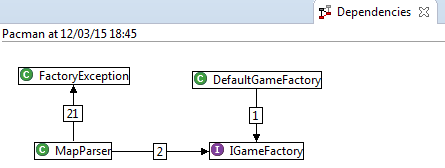
\includegraphics[width=\textwidth]{images/DependenciesFactory.png}
	\caption{\label{dependenciesF}Détail de l'analyse des dépendences cycliques du package Factory.}
\end{figure}

\begin{figure}[ht]
	\centering
	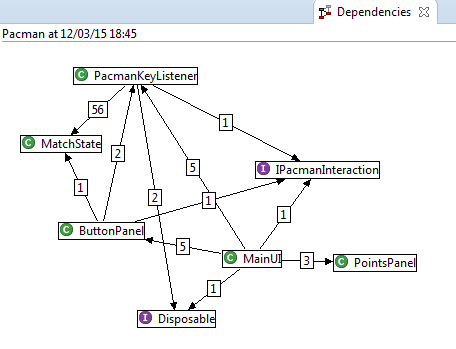
\includegraphics[width=\textwidth]{images/DependenciesUI.png}
	\caption{\label{dependenciesUI}Détail de l'analyse des dépendences cycliques du package UI.}
\end{figure}

\begin{figure}[ht]
	\centering
	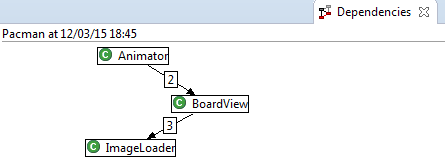
\includegraphics[width=\textwidth]{images/DependenciesVieuw.png}
	\caption{\label{dependenciesV}Détail de l'analyse des dépendences cycliques du package Vieuw.}
\end{figure}

\begin{figure}[ht]
	\centering
	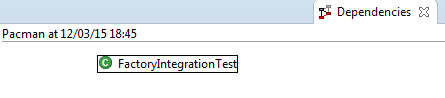
\includegraphics[width=\textwidth]{images/DependenciesFactoryTest.png}
	\caption{\label{dependenciesFT}Détail de l'analyse des dépendences cycliques du package Factory (Test).}
\end{figure}

\begin{figure}[ht]
	\centering
	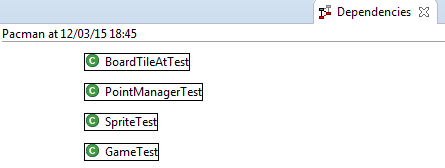
\includegraphics[width=\textwidth]{images/DependenciesModelTest.png}
	\caption{\label{dependenciesMT}Détail de l'analyse des dépendences cycliques du package Model (Test).}
\end{figure}

\begin{figure}[ht]
	\centering
	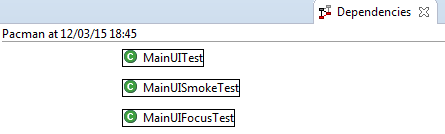
\includegraphics[width=\textwidth]{images/DependenciesUITest.png}
	\caption{\label{dependenciesUIT}Détail de l'analyse des dépendences cycliques du package UI (Test).}
\end{figure}

\begin{figure}[ht]
	\centering
	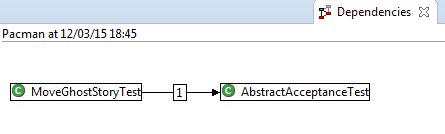
\includegraphics[width=\textwidth]{images/DependenciesAcceptTest.png}
	\caption{\label{dependenciesAT}Détail de l'analyse des dépendences cycliques du package Accept (Test).}
\end{figure}

\begin{figure}[ht]
	\centering
	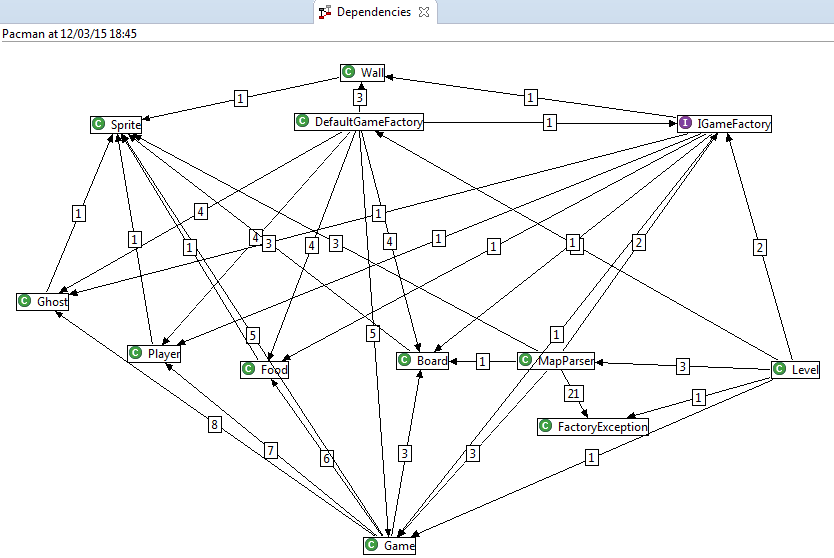
\includegraphics[width=\textwidth]{images/DependenciesModel_Factory.png} %images/DependenciesModel_Factory1.png
	\caption{\label{dependenciesMF}Détail de l'analyse des dépendences cycliques entre le package Model et la package Factory.} %avec en gras les classes du package Factory
\end{figure}


\clearpage
\newpage
\section{Annexe : ......}\label{InCode}

\begin{figure}[ht]
	\centering
	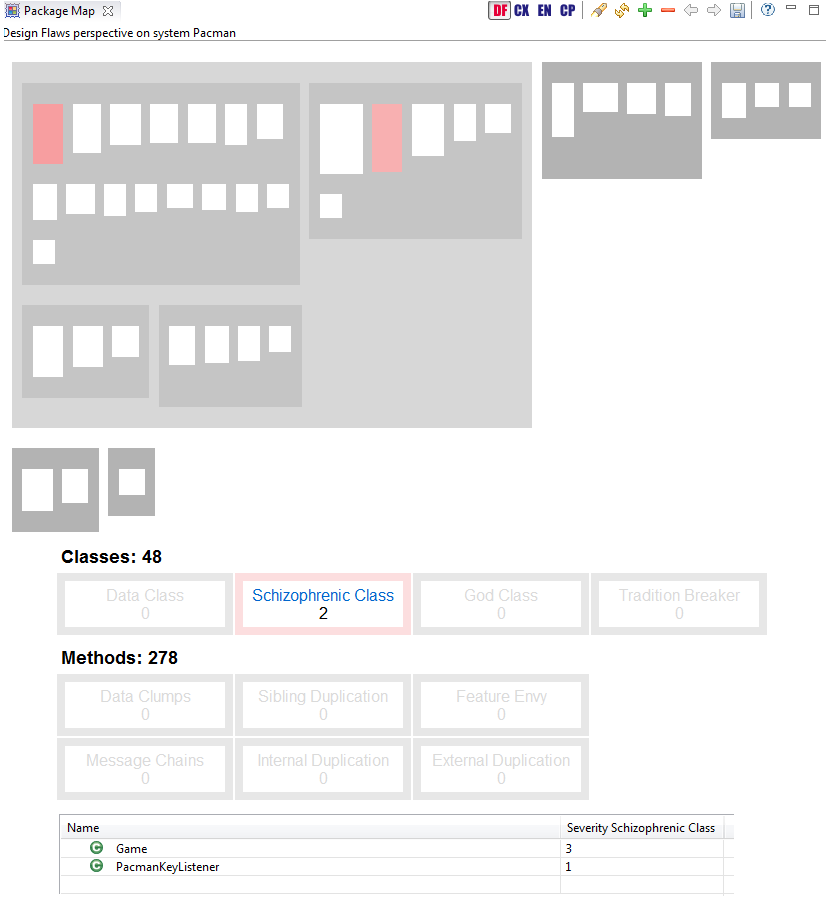
\includegraphics[width=\textwidth]{images/InCodeDesignFlaws.png}
	\caption{\label{incodeDF}Détail de l'analyse .........}
\end{figure}

\begin{figure}[ht]
	\centering
	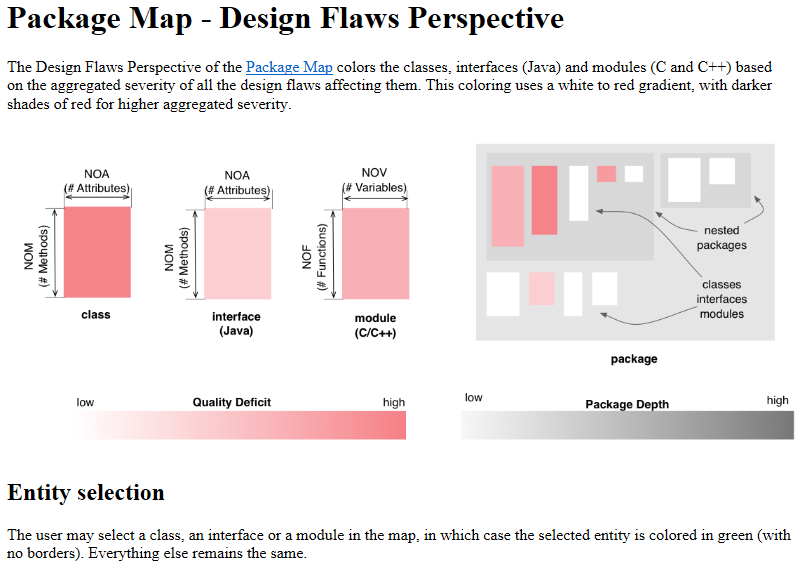
\includegraphics[width=\textwidth]{images/InCodeDesignFlawsLegende.png}
	\caption{\label{incodeDFLeg}Légende de l'analyse .........}
\end{figure}

\begin{figure}[ht]
	\centering
	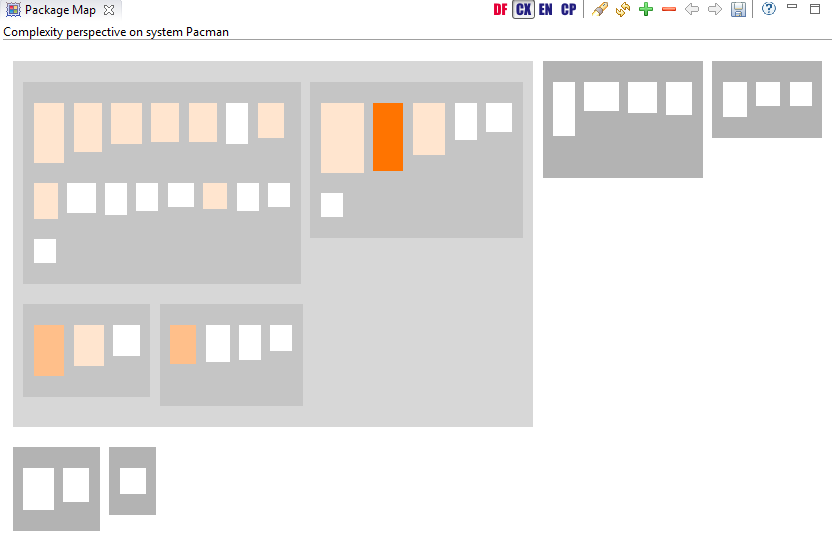
\includegraphics[width=\textwidth]{images/InCodeComplexity.png}
	\caption{\label{incodeCompl}Détail de l'analyse .........}
\end{figure}

\begin{figure}[ht]
	\centering
	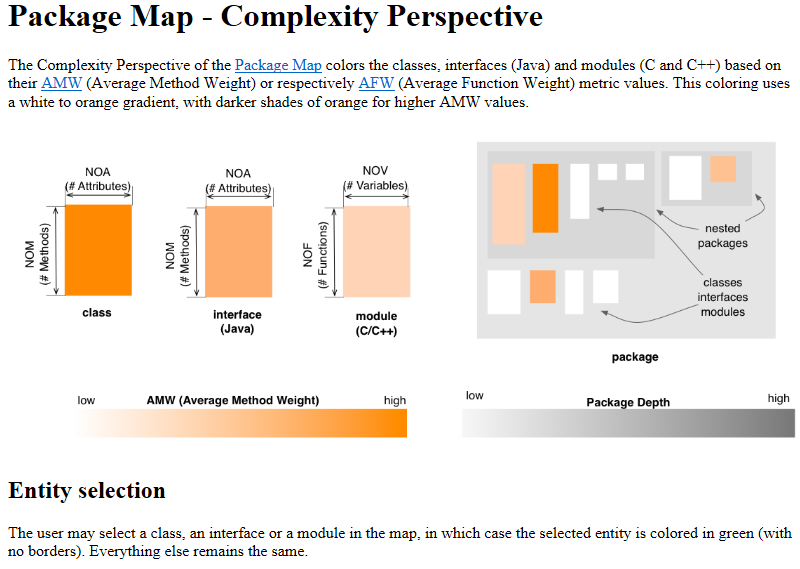
\includegraphics[width=\textwidth]{images/InCodeComplexityLegende.png}
	\caption{\label{incodeComplLeg}Légende de l'analyse .........}
\end{figure}

\begin{figure}[ht]
	\centering
	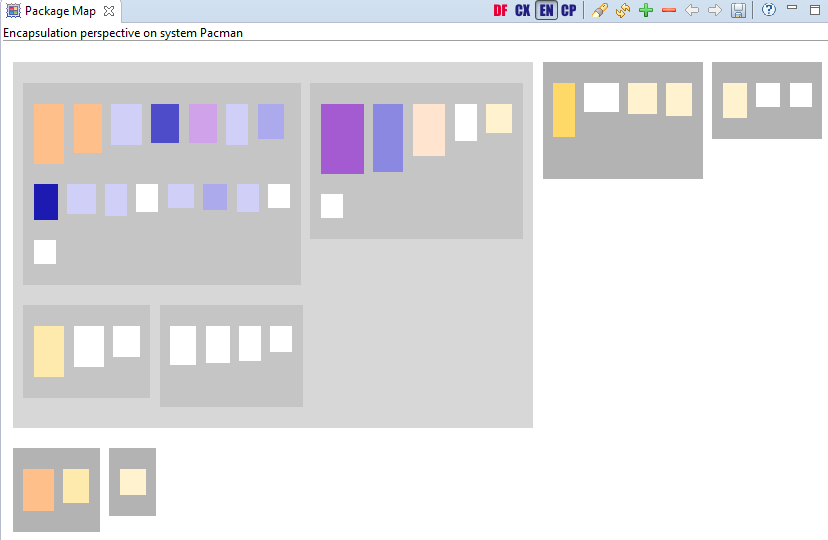
\includegraphics[width=\textwidth]{images/InCodeEncapsulation.png}
	\caption{\label{incodeEnc}Détail de l'analyse .........}
\end{figure}

\begin{figure}[ht]
	\centering
	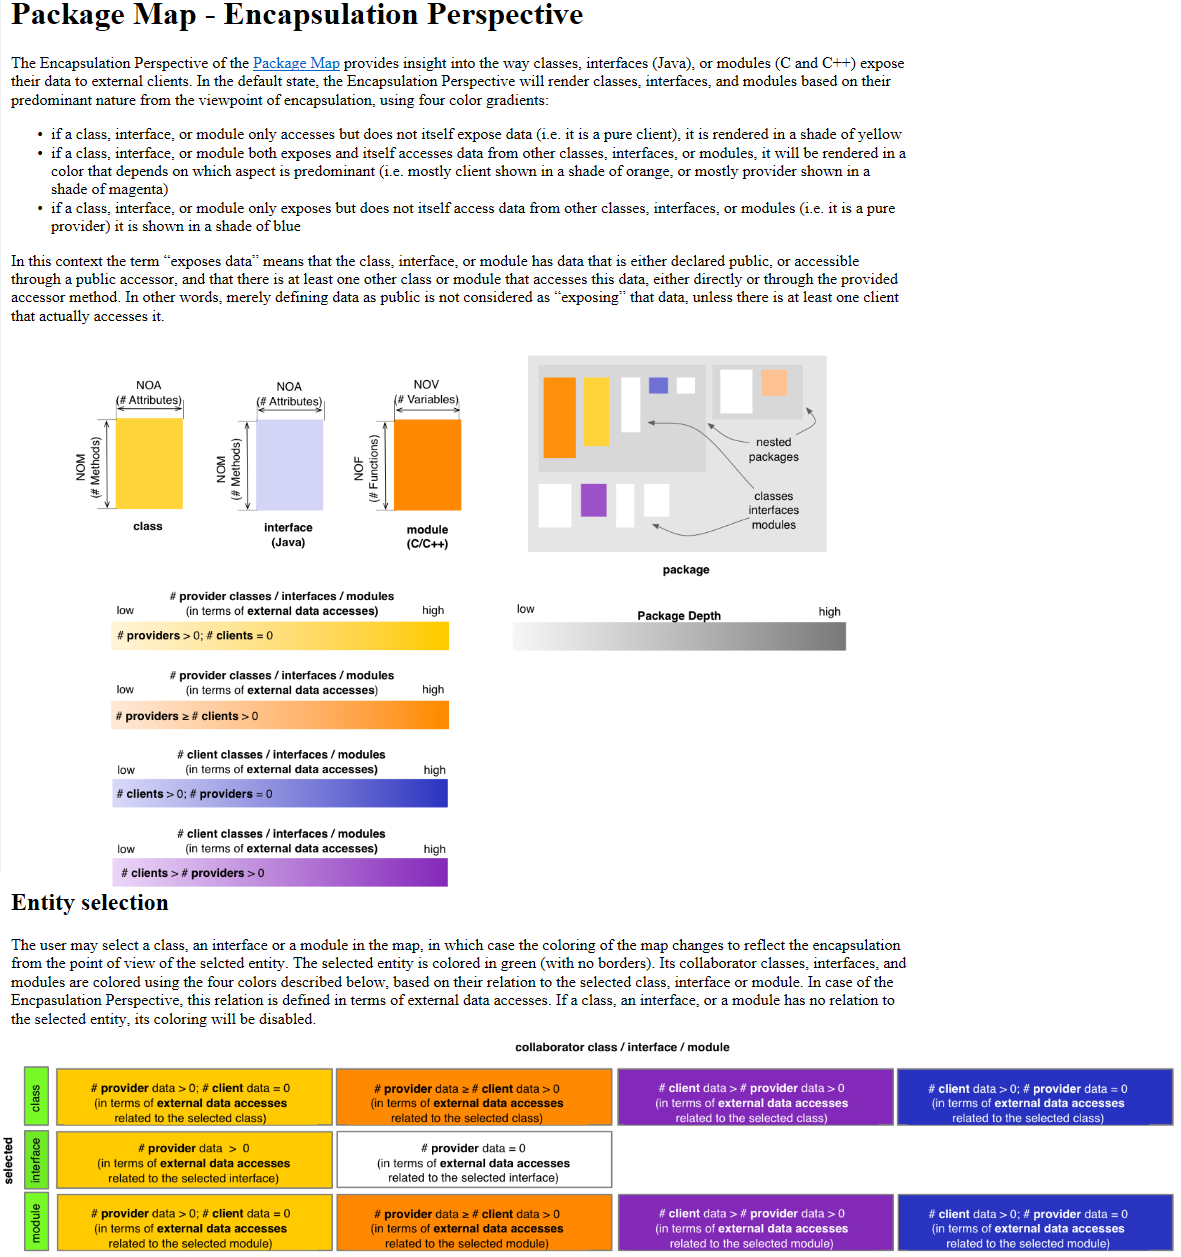
\includegraphics[width=\textwidth]{images/InCodeEncapsulationLegende.png}
	\caption{\label{incodeEncLeg}Légende de l'analyse .........}
\end{figure}

\begin{figure}[ht]
	\centering
	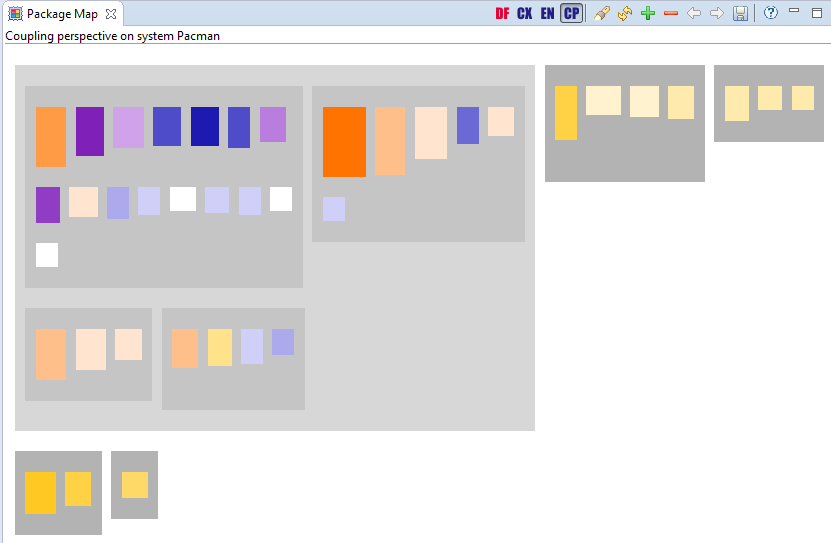
\includegraphics[width=\textwidth]{images/InCodeCoupling.png}
	\caption{\label{incodeCoupl}Détail de l'analyse .........}
\end{figure}

\begin{figure}[ht]
	\centering
	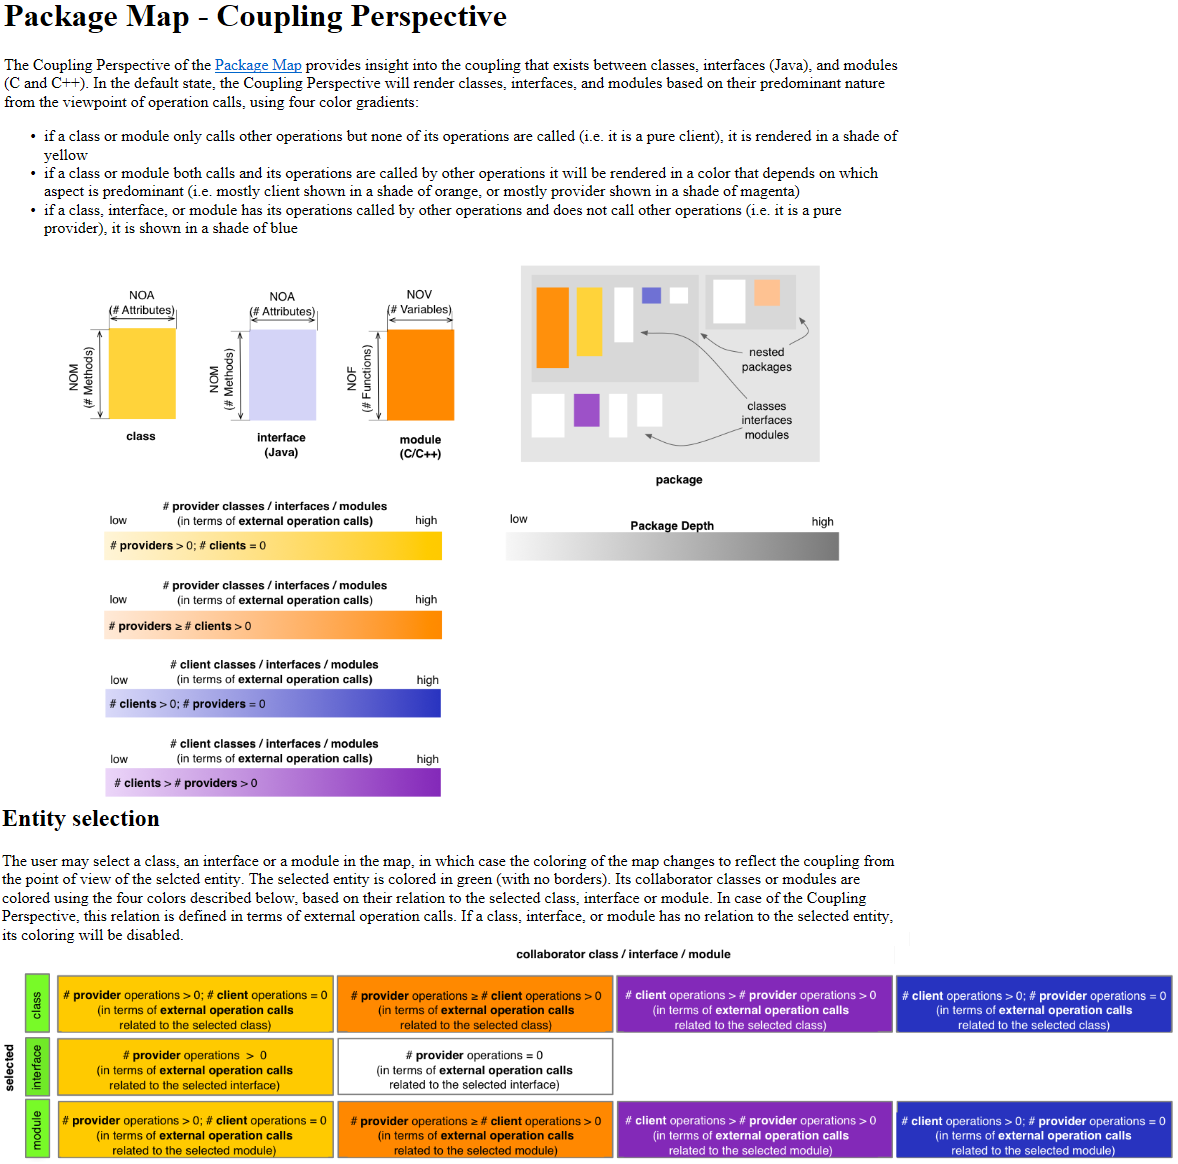
\includegraphics[width=\textwidth]{images/InCodeCouplingLegende.png}
	\caption{\label{incodeCouplLeg}Légende de l'analyse .........}
\end{figure}




\clearpage
\newpage
\section{Annexe : Couverture par les test}\label{coverage}

\begin{figure}[ht]
	\centering
	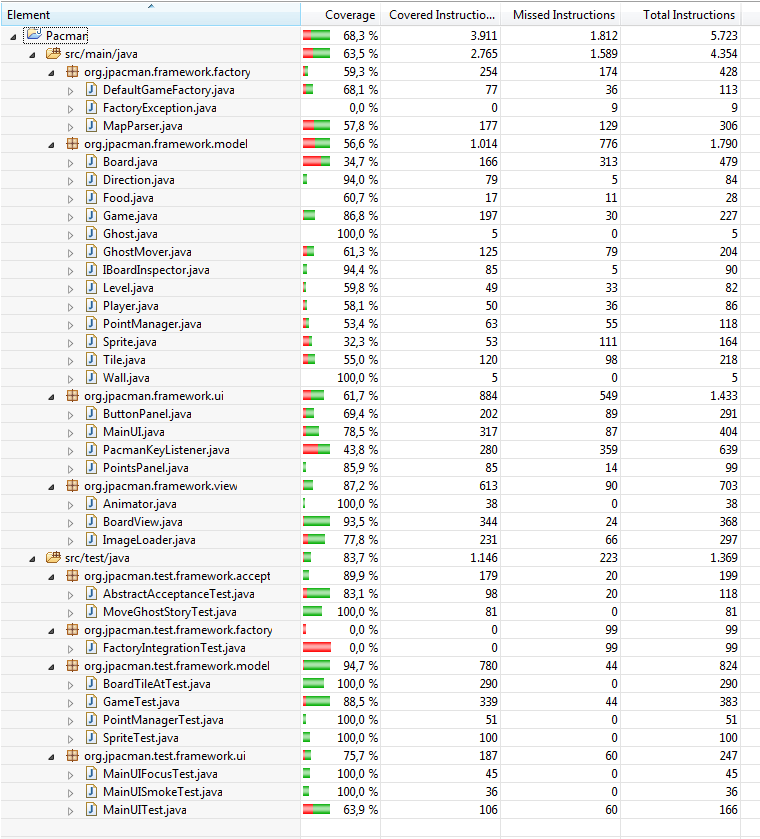
\includegraphics[width=\textwidth]{images/CoverageTest.png}
	\caption{\label{CoverageTest}Détail de l'analyse de couverture du code par les tests unitaires.}
\end{figure}


\begin{figure}[ht]
	\centering
	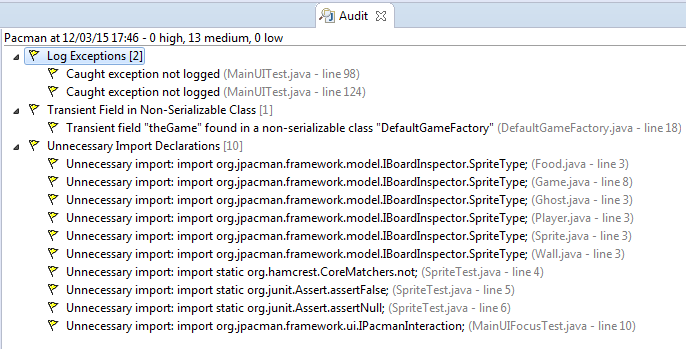
\includegraphics[width=\textwidth]{images/Audit.png}
	\caption{\label{Audit}Détail de l'analyse d'audit faite par Eclipse.}
\end{figure}


\newpage
\bibliographystyle{plain}
\bibliography{reference}

\end{document} 

